 %%\documentclass[12pt]{article}
 %\usepackage{epsfig}
%%  \textwidth 6.0in
 %% \textheight 9.2 in
 % \pagestyle{empty}
 %%\topmargin -0.25truein
%% \oddsidemargin -.6truein
%% \evensidemargin -.6truein
%% \parindent=1.5pc
%% \baselineskip=15pt

%%\newcommand{\oot}{\overline {126}}
%\documentclass[12pt]{article}	%%
%\baselineskip=7mm		%%
%\def\baselinestretch{1.2}	%%
%\usepackage[left=0.75in,top=0.6in,right=0.75in,bottom=0.6in]{geometry}


\documentclass[aps,onecolumn,showpacs,superscriptaddress,groupedaddress,nofootinbib,preprint]{revtex4-1}
\pdfoutput=1

\usepackage{slashed}
\usepackage{bm}        % for math
\usepackage{amssymb}   % for math
\usepackage{amsmath}
\usepackage{graphicx,psfrag,amsmath,subfigure}
\usepackage{booktabs}
\usepackage[colorlinks]{hyperref}
\usepackage{rotating}
\usepackage{units}
\usepackage{float}

\newcommand{\beqa}{\begin{eqnarray}}
\newcommand{\eeqa}{\end{eqnarray}}

\newcommand{\be}{\begin{equation}}
\newcommand{\ee}{\end{equation}}
\newcommand{\cl}{\%\,\,  \text{C.L.}}
\begin{document}
%\title{On finding collider-stable particles using Machine Learning}
\title{Collider searches for WIMP dark matter using Machine Learning}
\author{Charanjit K. Khosa, Veronica Sanz and Michael Soughton} 
%\email{V.Sanz@sussex.ac.uk}
%\email{ck373@sussex.ac.uk}
\affiliation{Department of Physics and Astronomy, University of Sussex, 
Brighton BN1 9QH, UK}
\date{\today}
\begin{abstract}
We study the WIMP dark matter searches using supervised machine learning techniques. 
Prospects of detecting WIMP monojet signal over the SM background are considered. We compare the performance of 
various ML algorithms and propose new scheme to average over many events. By using the 2D images there is a gain in the performance.
We also address the question what is the probability that other dark matter signals may look like WIMP dark matter. For the other signals 
we consider, axion like particles and monojet production in the effective field theory set-up. We perform analysis for both parton level and detector level simulations.
\end{abstract}
\maketitle 

\section{Introduction}
\noindent Collider searches for Dark Matter (DM) are one of the most important avenues for New Physics searches at the Large Hadron Collider (LHC). Typical searches include the identification of singular objects within the detector (mono searches), where single object could be a jet, W, top quark, Higgs boson, photon or $ t \bar t $ pair. The motivation for using these channels is that DM candidates (which cannot be directly detected) could be exposed through a momentum-mismatch in the final state where the detected objects appear to recoil against nothing. Like other new physics searches at the LHC, these channels face high levels of SM backgrounds, however they also face the possibility of contamination by other collider stable particles.
\\
\\
WIMP DM motivation and status...
\\
\\
Collider stable particles are any particles which do not interact with the detector and do not decay before leaving it, hence manifesting as missing momentum, mimicking Dark Matter particles. Note that a collider stable particle could be completely stable (as is thought to be the case for DM particles) or be unstable but with a lifetime long enough such that it is not likely to decay before it leaves the detector. In our search for new physics at the LHC, we must then attempt to remove this degeneracy. This task is even more challenging than analysing the signal and background for DM searches because here we are concerned with two or more (unknown) physics models. 

END
\\
\\

WIMP dark matter motivation and status...
%Collider stable particles could manifest themselves as missing momentum, mimicking dark matter particles. This task is even more challenging than
% analyzing the signal and background for the DM searches because here we are concerned with the two or more(unknown) new 
% physics models. The decay width of the particle is a parameter of its mass which we do not know a priori. In this situation, one would like to 
% design a search template with respect to the better understood new physics model. This complex analysis certainly requires the implementation 
% of new (more sophisticated) techniques beyond  conventional search strategies. This calls for the use of machine learning algorithms which are 
% emerging as a suitable platform for exploring a co-relations in multi-dimensional parameter space.
At present, LHC dark matter searches are interpreted using simplified dark matter models

Recent papers: DM searches using ML (ALPs paper,

In this work, we consider monojet process and use Machine Learning to compare the features of dark matter(DM) signals from BSM models. Specifically 
WIMP dark matter, Axion-Like Particles (ALPs) Effective Field Theory \cite{Mimasu:2014nea,Brivio:2017ije} and a simplified DM model with a
spin-1 mediator [2]. 

Paper is organised as follows:

\begin{figure} [H]
\centering
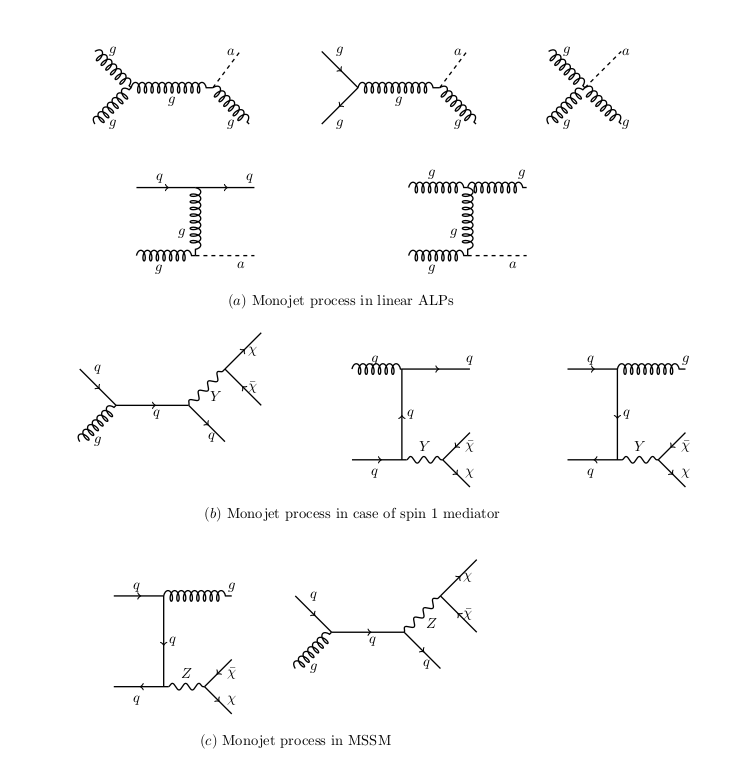
\includegraphics[scale=0.35]{draftfig/fyndiag.png}
\caption{Feynman diagrams for mono-jet process in Linear ALPs case, spin 1 mediator and in MSSM\label{fyndiag}.}
\end{figure}

\section{Kinematic distributions for the benchmark processes}
For the signal, we consider three cases; (1) when dark matter candidate is collider stable particle (2) when dark
matter is produced from the decay of the heavy mediator, (3) weakly interacting massive particle in the R-parity conserving supersymmetric
scenario. Feynman diagrams for the mono-jet process in these cases are shown in Figure \ref{fyndiag}.
%\subsection{WIMP : Susy}
%\subsection{Axion like particles}
Axions like particles(ALPs) is the 
typically example of collider stable particles. ALPs could be present in many theoretically well motivated models. Depending on 
the model details, different mass and coupling range is possible for these particles. ALPs themselves could be dark matter particle\cite{} or
 can be a dark matter mediator. These exotic particles are constrained by many collider searches in addition to 
 the astrophysical constraints. In fact, collider constraints are complementary to the astrophysical constraints\cite{}. The direct 
 axion search experiments are designed to target their couplings with the photons. ALPs could look like MET if they decay outside the detector volume.
 
The effective Lagrangian for linear ALPs could be written as:
\begin{align}\label{eqn:L_eff}
    \mathcal{L}_a = &\frac{1}{2}\partial_{\mu}a\,\partial^{\mu}a  - \frac{1}{2}M_{a}^2 a^2
                  -\frac{g_{a\gamma}}{4}a\,F_{\mu\nu}\tilde{F}^{\mu\nu} \nonumber 
                   - \frac{g_{agg}}{2}a\,\text{Tr}\left[G_{\mu\nu}\tilde{G}^{\mu\nu}\right] 
                  +\sum_{\psi}g^{\psi}_{a} \,m_\psi\,a\bar \psi \gamma^5 \psi\,,
                   % +\,ig_{ah}\left(\Phi^{\dagger}\overleftrightarrow{D}_{\mu}\Phi\right)\partial^{\mu}a\,,
\end{align}
ALP-gluon coupling \cite{Mimasu:2014nea,Brivio:2017ije} :
\[
g_{agg} \lesssim \unit[1.1\cdot10^{-5}]{GeV^{-1}} \quad (90\cl) \quad \text{for}\quad m_a \lesssim \unit[60]{MeV}\,.
\]

\[ f_a=1\,\, \mbox{TeV} \quad \quad  M_{a}=1\,\, \mbox{MeV}  \]

\begin{figure} [H]
\begin{center}
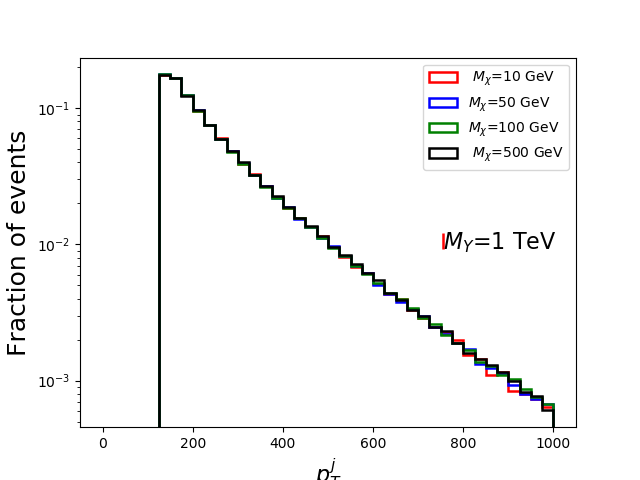
\includegraphics[scale=0.40]{draftfig/ptjS1med1tev.png}
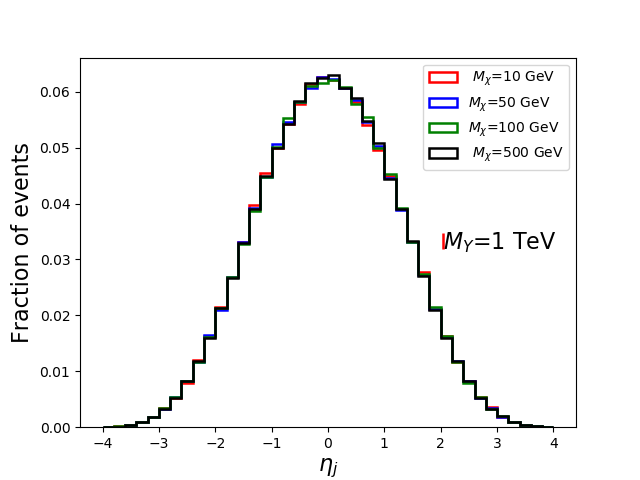
\includegraphics[scale=0.40]{draftfig/etajS1med1tev.png}
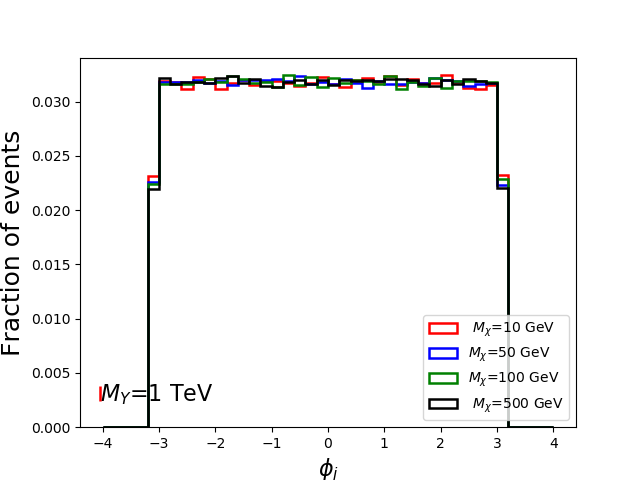
\includegraphics[scale=0.40]{draftfig/phijS1med1tev.png}
\caption{The $p_T$, $\eta$, $\phi$ distributions for the monojet  in case of EFT spin-1 mediator (at parton level) for fixed mediator mass and 
varied dark matter mass\label{spin1med}.}
\end{center}
\end{figure}

%\subsection{Simplified Models : Spin 1 Mediator}
We focus on the heavy mediator case. Once the mediator is heavy enough to produce the 
dark matter then kinematics is not very sensitive to the dark matter mass as shown in Fig. \ref{spin1med}. For further analysis, we use 
 $M_Y=1\,\, \mbox{TeV}$ and  $M_{\chi}=10\,\, \mbox{GeV}$ mass parameters.



\begin{figure} [H]
\centering
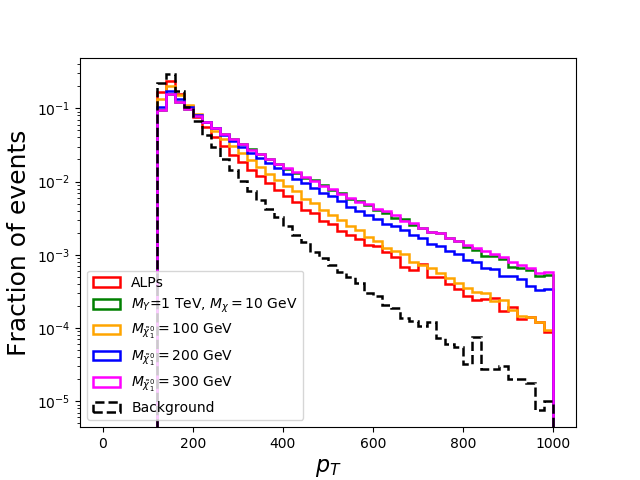
\includegraphics[scale=0.40]{draftfig/ptjallsb.png}
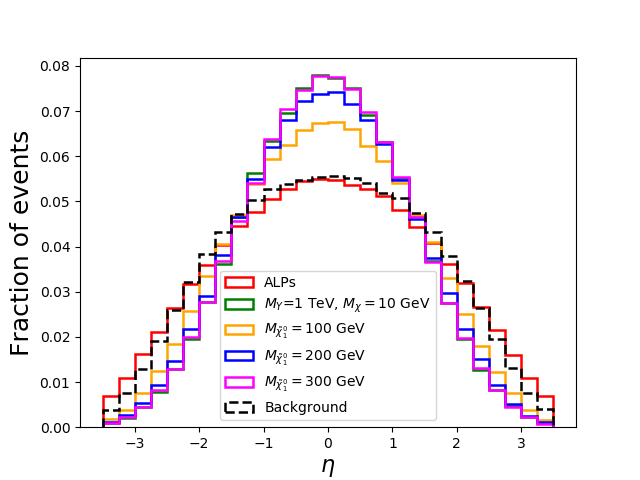
\includegraphics[scale=0.40]{draftfig/etajallsb.png}
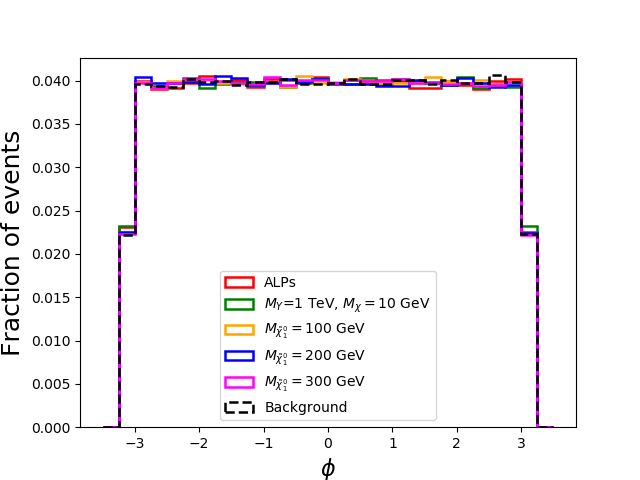
\includegraphics[scale=0.40]{draftfig/phijallsb.png}
\caption{The 1D histograms for the monojet process for linear ALPs, spin-1 mediator case, WIMP and SM background for the LO parton level simulation.\label{1Dand2DfeaturesPL1}}
\end{figure}


\begin{figure}% [H]
\centering
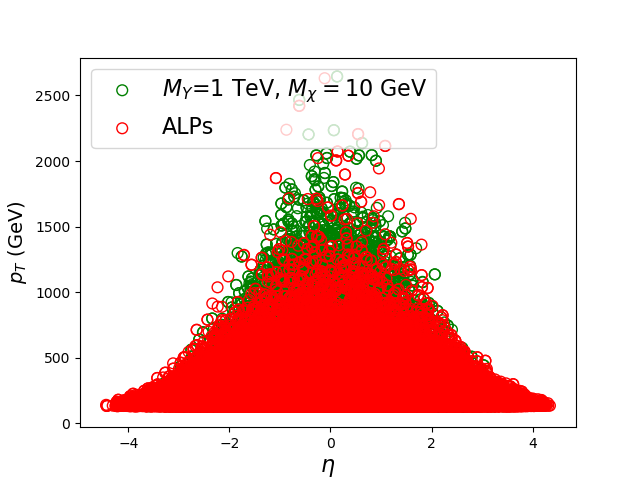
\includegraphics[scale=0.32]{draftfig/ptjetajaxspin1.png}
%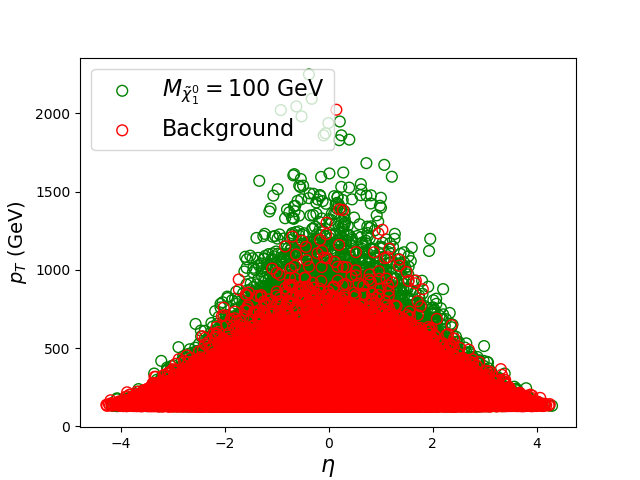
\includegraphics[scale=0.32]{draftfig/ptjetajsmsusy1.png}
%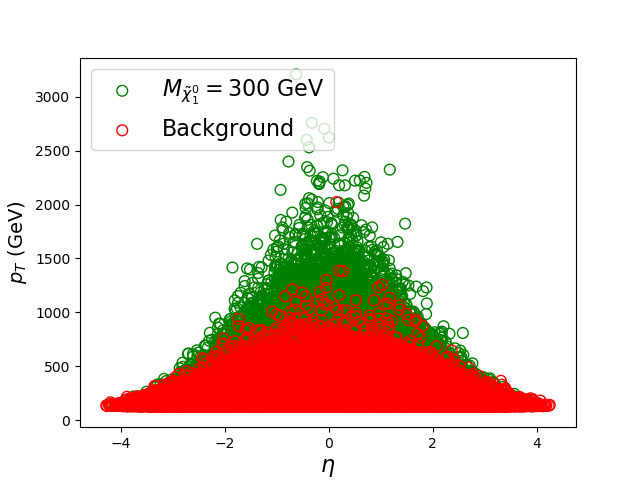
\includegraphics[scale=0.32]{draftfig/ptjetajsmsusy3.png}
%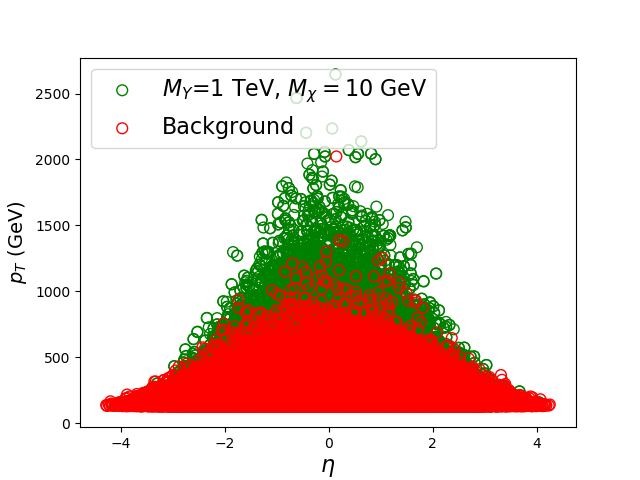
\includegraphics[scale=0.32]{draftfig/ptjetajsmeft.png}
%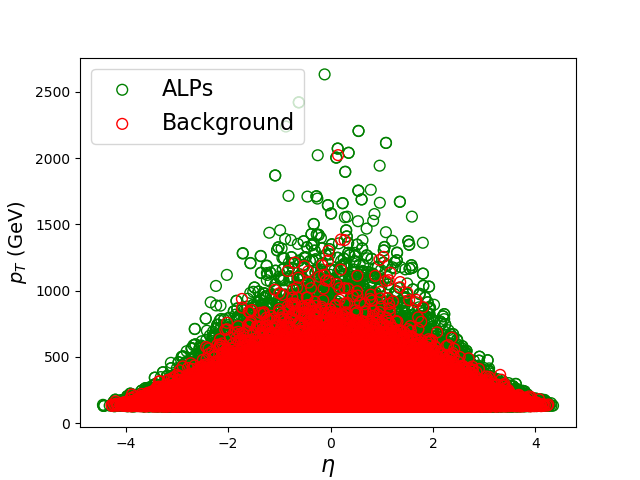
\includegraphics[scale=0.32]{draftfig/ptjetajsmaxion.png}
%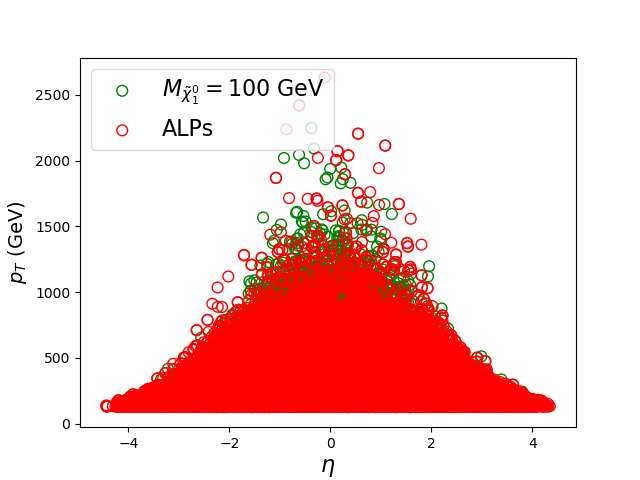
\includegraphics[scale=0.32]{draftfig/ptjetajaxsusy1.png}
\caption{2D histograms for the monojet process for several combinations of signals and signal  versus SM background for the LO parton level simulation.\label{1Dand2DfeaturesPL2}}
\end{figure}




\begin{figure} [H]
\centering
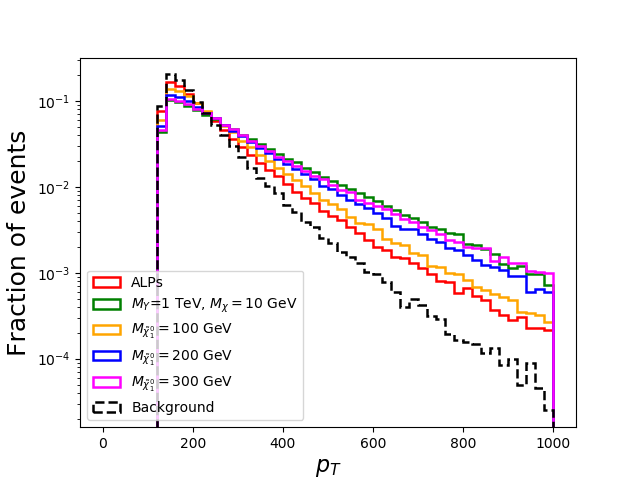
\includegraphics[scale=0.40]{draftfig/ptjallsbdelphes.png}
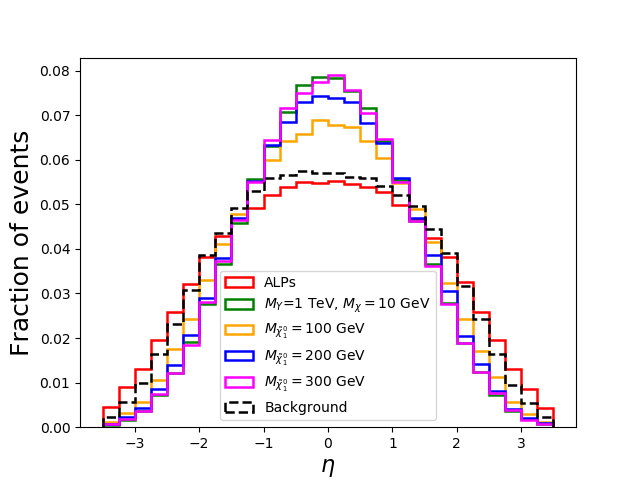
\includegraphics[scale=0.40]{draftfig/etajallsbdelphes.png}
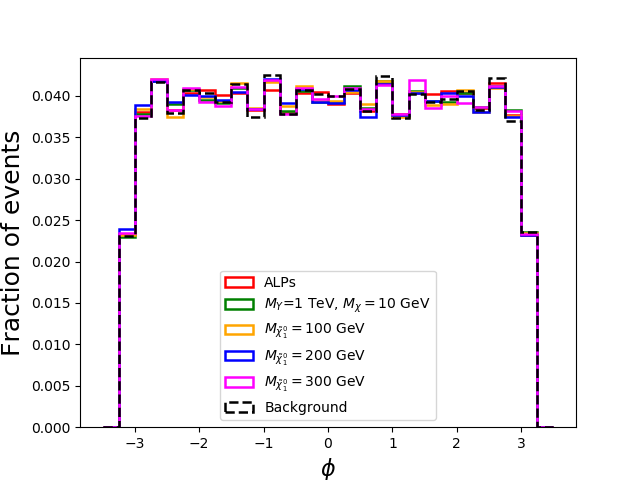
\includegraphics[scale=0.40]{draftfig/phijallsbdelphes.png}
\caption{1D histograms for the monojet process for linear ALPs, spin-1 mediator case, WIMP and SM background (detector simulation).\label{1Dand2DfeaturesDL}}
\end{figure}

We perform both parton level and detector level simulation to generate the data sample. More details related to event 
generation can be found in Appendix \ref{setup}. The kinematic features for parton level monojet process and detector 
level event generation are shown in Figure \ref{1Dand2DfeaturesPL1},\ref{1Dand2DfeaturesPL2} and \ref{1Dand2DfeaturesDL} respectively.
 The transverse momentum and $\eta$ of monojet process inALPs are very similar to that of SM background. There is no preferred direction of $\phi$ for all 
 the signal and SM background process.
\section{DM signal detection using machine learning}
We used the supervised machine learning techniques for the dark matter signal classification.
\subsection{Logistic regression} 
At the first step, we do logistic regression for the monojet data. We used SGDclassifier of sklearn library with log loss function. Data sample is divided as 
70$\%$ $:$ 30$\%$ for training sample and test sample. The balanced data set is considered for both the classes. ROC curves for the all the  signals are shown in figure \ref{rocLO-LR-NN}. We can see that AUC varies from 0.58 to 0.71 for the ALPs and SUSY BP3 case and 
other 3 cases lie in between. One can easily separate heavy WIMPs from the Z$+$jet SM background however ALPs monojet could not be efficiently classified.
The regularization parameter $\lambda= 10^{-5}$ is used for all the cases.



\begin{figure}% [H]
\centering
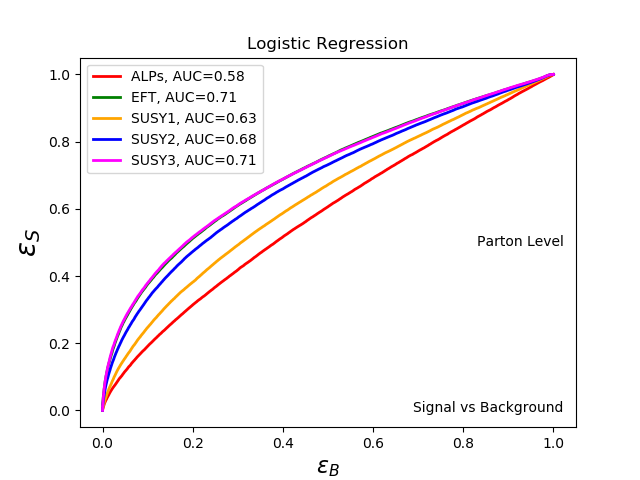
\includegraphics[scale=0.50]{draftfig/ROCsbLR.png}
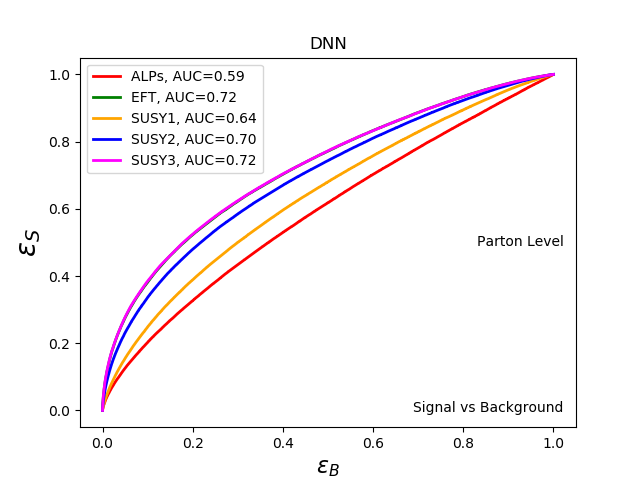
\includegraphics[scale=0.50]{draftfig/ROCsbNN.png}
\caption{ROC curves using logistic regression (left panel) and neural network with 5 hidden layers (right panel) for different signals versus background for the LO parton level analysis. 
%For NN code, I used only two features, $p_T^j$ and $\eta^j$
}\label{rocLO-LR-NN}
\end{figure}


\begin{figure}% [H]
\centering
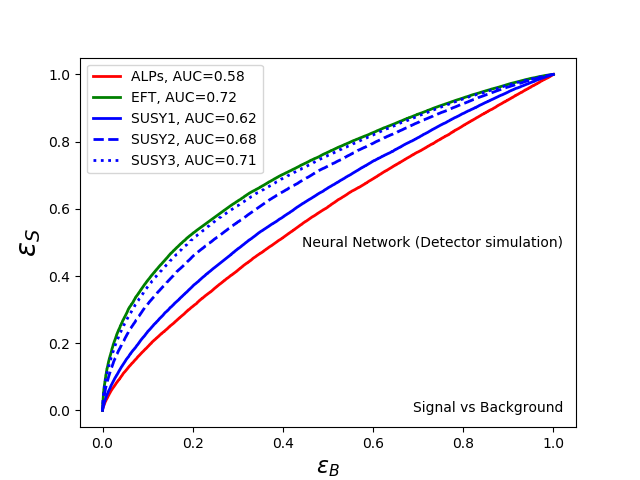
\includegraphics[scale=0.50]{draftfig/ROCsbNNdelphes.png}
\caption{ROC curves using neural network with 5 hidden layers for different signals versus background for the LO detector level simulated data. 
%For this I  used only all three features, $p_T^j$, $\eta^j$, $\phi^j$ 
}\label{roc-LOdelphes-NN}
\end{figure}

\subsection{Neural Network-kinematic features}
We investigate the classification accuracy using  neural networks (NN) with the same input 
features i.e. $p_T$ and $\eta$ of the jet. We used 5 (fully connected) hidden layers for the  network as including more 
layers does not improve the performance. For the intermediate layers, ReLU activation function is used and we considered binary cross entropy loss function.
For the parton level event generation, we show the ROC curves for various signals in right panel of figure \ref{rocLO-LR-NN}. The classification accuracy for the 
detector level event generation is also compared in figure \ref{roc-LOdelphes-NN}.  In figure \ref{roc-LO-PL-delphes-NN}, we 
compare the ROC curves for parton level and detector level data sample. The difference in both the cases is very small.


\begin{figure} %[H]
\centering
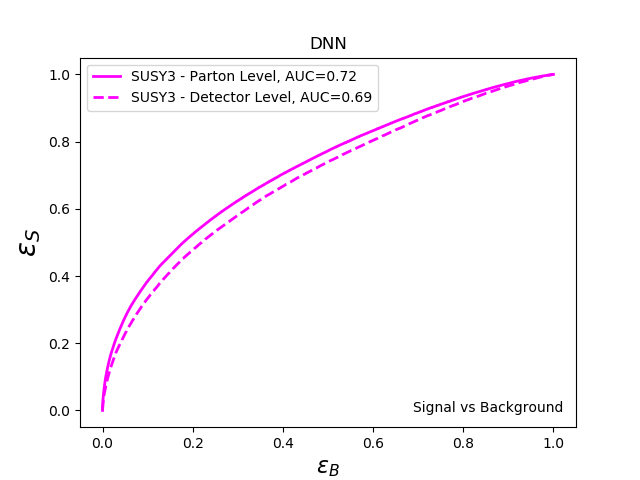
\includegraphics[scale=0.50]{draftfig/ROCsbNNcomparePLandDelphes.png}
\caption{ROC curves (neural network with 5 hidden layers) for SUSY BP1 versus background for parton level and detector level simulation.}\label{roc-LO-PL-delphes-NN}
\end{figure}

\subsection{NN-2D histograms}
Inspired by the use of Convolutional Neural Networks (CNNs) in the classification of images, we construct 'images' from 2D histograms using $p_T$ and $\eta_j$ of the jet and by dividing the simulated dataset which contains $N_\text{Tot}$ total number of events into $N_\text{Images}$ number of images, such that each image contains $N$ number of events. CNNs offer the possibility of learning additional information from spatial features of data such as edge detection. However in our case we find that CNNs gain little information since the input data are not real images with patterns arising form complex real world phenomenon but rather histograms with features already encoded through the distributions ($p_T$ and $\eta$) used to make them. Regardless, the method of creating a number of 'images' to train a network on on is still a powerful since each image is itself giving an approximation of the joint probability density function distribution for both $p_T$ and $\eta$ and there are also many images to train over. The degree to which each image approximates the joint probability density function depends on the number of events $r$ chosen to be in an image. For a fixed total number of events the will then be a trade-off between $r$ and $N_\text{images}$ that will affect the accuracy of the model DISCUSS OF HERE OR LATER? 

Before analysing the data with a CNN, we first attempt solving the problem with a DNN. This is achieved by decomposing the 2D histogram into a 1D array with values corresponding to the normalised number of events in each bin. Note that whilst the may seem like we are just reconstructing the original distributions, this is not the case since this data now contains a correlation between from individual distributions. A few illustrative pictures of these plots are shown in figure \ref{demopic}. We consider $p_T$ and $\eta$ in range [100, 2000] GeV and [-4 to 4], respectively with 29 $\times$ 29 bins. We use the information of event density in this grid as an input for a DNN. The network is well optimised with two fully connected hidden layers, both consisting of twenty neurons with a ReLU activation function and a softmax activation function for the output layer. We do not find overtraining to be a serious issue here so only include a small number of dropout neurons. The network is trained for 30 epochs with a batch size of 50. We evaluate the network performance through accuracy (found from finding whether the predicted result (ranging from 0 to 1) round to 0 or to 1) - this is done within the training dateset whilst training, then with the validation dataset whilst evaluating the how the network is training and finally with the test dataset. In figure \ref{accuracy1}, we show the performance dependence on the number of events injected in one picture for the fixed data sample. 
The different colored curves correspond to varying total data sample. More explicitly, for the fixed data sample, the number of data points NN is trained and tested is 
less in the case where we have more events per image.
\begin{figure} [H]
\centering
\includegraphics[scale=0.40]{draftfig/pic1susybp1200events.png}
\includegraphics[scale=0.40]{draftfig/pic2susybp1200events.png}
\includegraphics[scale=0.40]{draftfig/pic1axion200events.png}
\includegraphics[scale=0.40]{draftfig/pic2axion200events.png}
\caption{Illustrative 2D histograms for SUSY BP1 (upper row) and ALPs case (lower row) averaging over 200 events.}\label{demopic}
\end{figure}


\begin{figure}% [H]
\centering
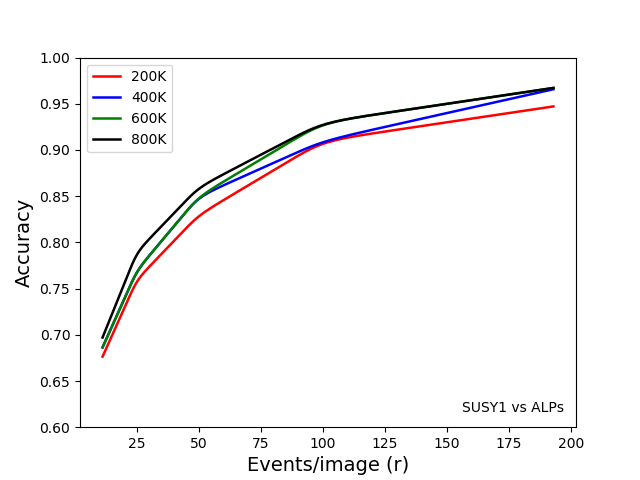
\includegraphics[scale=0.40]{draftfig/accuracyplot2dSUSY1vsAxion.pdf}
\caption{Accuracy versus no events per images with the varying number of events for WIMP BP1 versus ALPs using fully connected NN with 2 hidden layers. Red, blue,
green and black curves corresponding to a data sample of 200K, 400K, 600K, and 800K events.NEED TO REPLACE THIS FOR SIGNAL VS BACKGROUND.} \label{accuracy1}
\end{figure}
THIS WILL GO IN AN EARLIER SECTION: We simulate detector level events using Delphes and Pythia8 CITE AND WRITE PROPERLY WITH VERSION. For this analysis we will consider only the kinematics of the leading jet. CUTS. We then perform the analysis as was done for the parton level simulation, constructing 2D histograms of $p_T^{j_{\text{leading}}}$ and $\eta^{j_{\text{leading}}}$. The ROC curves for signal to background identification using DNNs with the 2D histograms for $r=20$ are shown to the right in Figure \ref{2D_DNN_sig_vs_bg_LO_ROC} the ROC curves for signal to signal identification are shown to the right in Figure \ref{2D_DNN_sig_vs_sig_LO_ROC} .
\begin{figure}% [H]
\centering
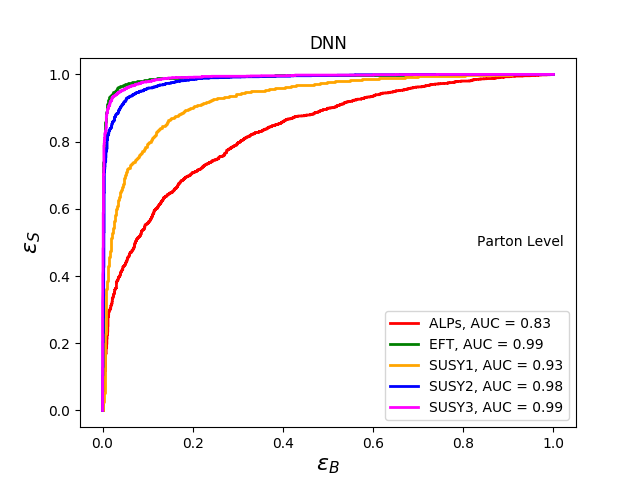
\includegraphics[scale=0.50]{draftfig/2D_DNN_sig_vs_bg_LO_ROC.png}
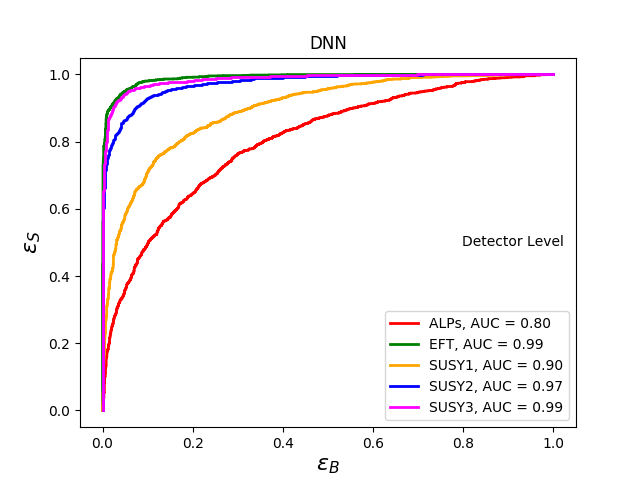
\includegraphics[scale=0.50]{draftfig/2D_DNN_sig_vs_bg_delphes_ROC.png}
\caption{ROC curves (DNN with 2D histograms, $r = 20$) for signal versus background for the parton level (left panel) and detector level simulation (right panel). For these plots, 100K events are used for each process in both the cases.}\label{2D_DNN_sig_vs_bg_LO_ROC}
\end{figure}

\begin{figure}% [H]
\centering
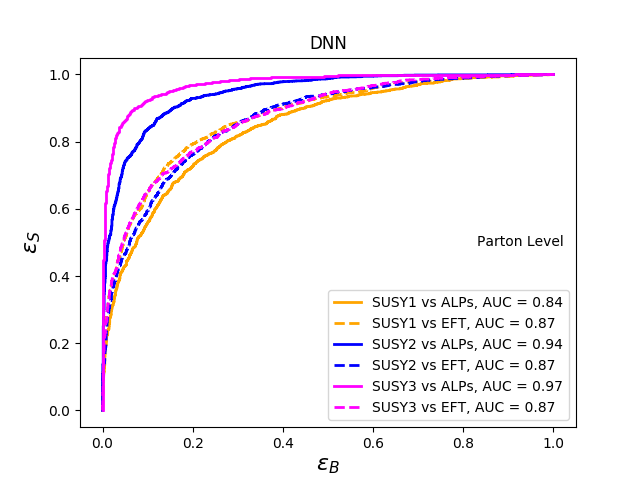
\includegraphics[scale=0.50]{draftfig/2D_DNN_SUSY_vs_sig_LO_ROC.png}
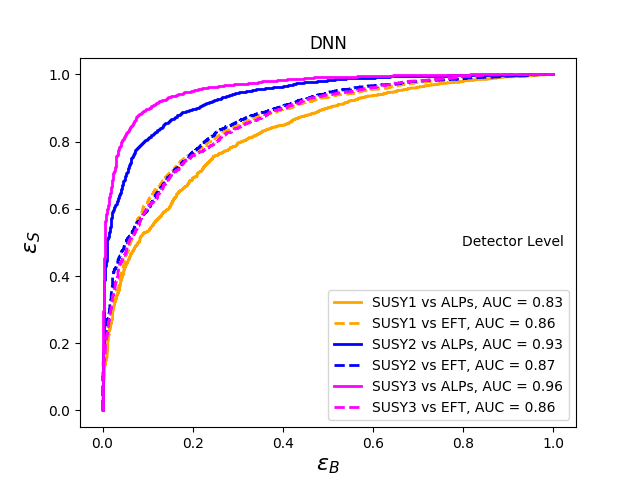
\includegraphics[scale=0.50]{draftfig/2D_DNN_SUSY_vs_sig_delphes_ROC.png}
\caption{ROC curves (DNN with 2D histograms, $r = 25$) for SUSY benchmarks versus other signals for the parton level(left panel) and detector level simulation (right panel).}\label{2D_DNN_SUSY_vs_sig_LO_ROC}
\end{figure}


We also consider the Next-to-Leading-Order (NLO) processes in which two parton level jets are produced. We simulate detector level - THE DATASETS ARE WITH DELPHES CORRECT? datasets for the NLO processes and now take the leading jet as well as the jet with the second highest transverse momentum (note that there is the possibility of the second jet arising from a showering process from this first jet and not being the original second jet, however we do not believe that this should affect our analysis since this would be a rare occurrence and a ML algorithm will still find patterns in the data regardless of the origin of the jet). <-- THIS SHOULD GO IN THE PREVIOUS SECTION 
\\
\\
Since for the NLO process we have 8 different features: $ p_T^{j_1}, p_T^{j_2}, \eta_{j_1}, \eta_{j_2}, MET, \Delta \phi_{jj}, \Delta \phi_{MET j_1},$ $\Delta \phi_{MET j_2}, $ there are 28 possible variations of 2D histograms that we could produce. If this was to be done then it might prove fruitful to combine the results of those 28 ML algorithms together in some manner. Alternatively one could produce 3 (or higher)-dimensional histograms and deconvolve them for the DNN or use a 3 (or higher)-dimensional CNN, however we shall not take this approach here for risk of overcomplicating an analysis which may not benefit from it. Instead we perform a Principal Component Analysis (PCA) to the NLO data in order to determine which features are more relevant. Figure \ref{PCA_plots} shows that most of the variance within the datasets is captured within the first three principal component axes. By finding the correlation between the original features and the new principal component axes, we can determine which features are most important in terms of holding information. The correlations can be seen in Table \ref{PCA_table} in Appendix \ref{PCA}. One can see from the table that the most important three features varies by dataset (all features except all features except $p_T^{j_2}$ and $\Delta \phi_{\text{MET}}^{j_2}$ occur amongst the top three in at least one dataset).
\begin{figure}% [H]
\centering
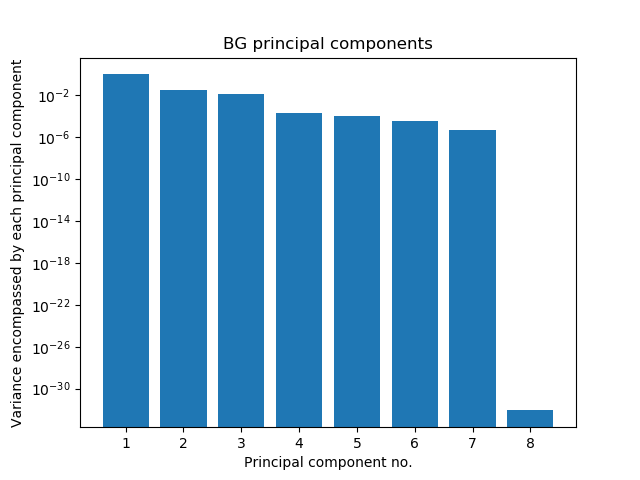
\includegraphics[scale=0.32]{draftfig/BG_PCA.png}
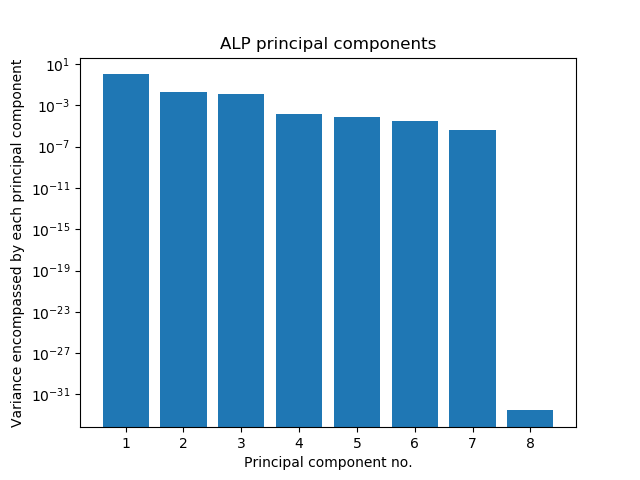
\includegraphics[scale=0.32]{draftfig/ALP_PCA.png}
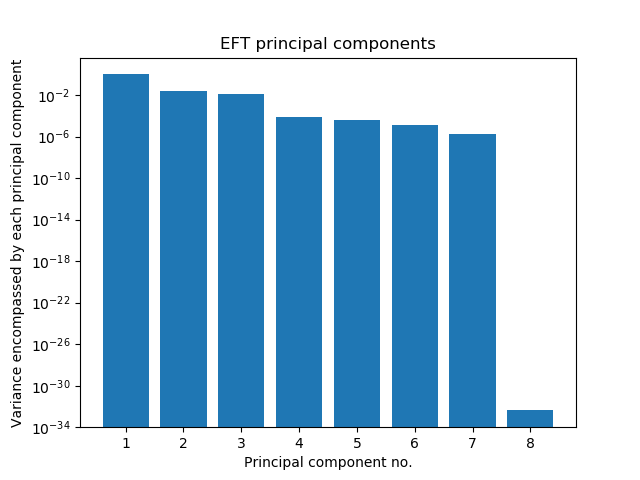
\includegraphics[scale=0.32]{draftfig/EFT_PCA.png}

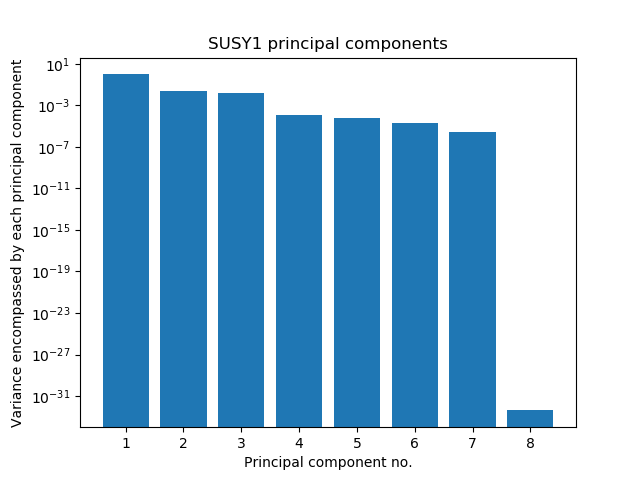
\includegraphics[scale=0.32]{draftfig/SUSY1_PCA.png}
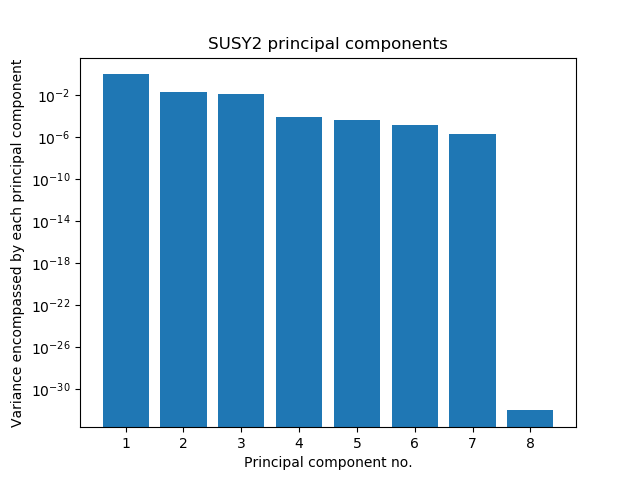
\includegraphics[scale=0.32]{draftfig/SUSY2_PCA.png}
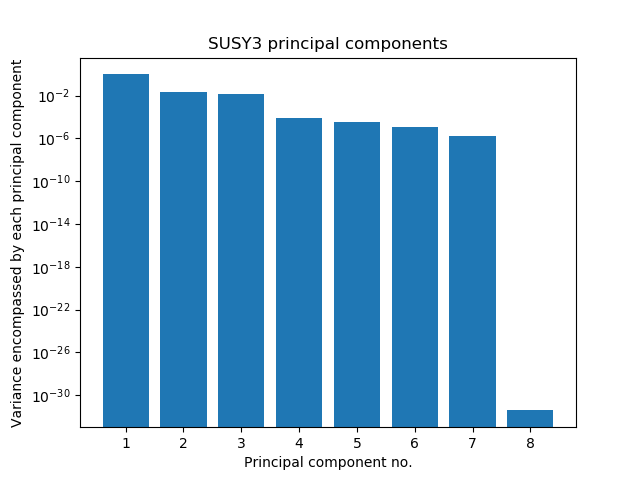
\includegraphics[scale=0.32]{draftfig/SUSY3_PCA.png}
\caption{The explained variance ratio of the new principal component axes (with the number of principal component axes being 8, the same number of original features), highlighting the relative importance of the principal components in terms of capturing variance in the datasets}\label{PCA_plots}
\end{figure}

We shall use $p_T^{j_1}$ and $\Delta \phi_{\text{MET}}^{j_1}$ to construct 2D histograms since they are the two features which occur the most amongst the top two principal components, however one could gain from including the other features as well. We do find an increase in classifier performance when using these two distributions over $p_T^{j_1}$ and $\eta_{j_1}$. The ROC curves for a DNN (with the same architecture as before) are shown in Figures \ref{2D_DNN_sig_vs_bg_NLO_ROC} (signal-to-background) and \ref{2D_DNN_sig_vs_sig_NLO_ROC} (signal-to-signal).

\begin{figure}% [H]
\centering
\includegraphics[scale=0.50]{draftfig/2D_DNN_sig_vs_bg_NLO_pt-metphij1_ROC.png}
\caption{ROC curves (DNN with 2D histograms, $r = 20$) for signal versus background for the dijet NLO detector level simulation. For these plots, 40K events are used for each process in both the cases.}\label{2D_DNN_sig_vs_bg_NLO_ROC}
\end{figure}

\begin{figure}% [H]
\centering
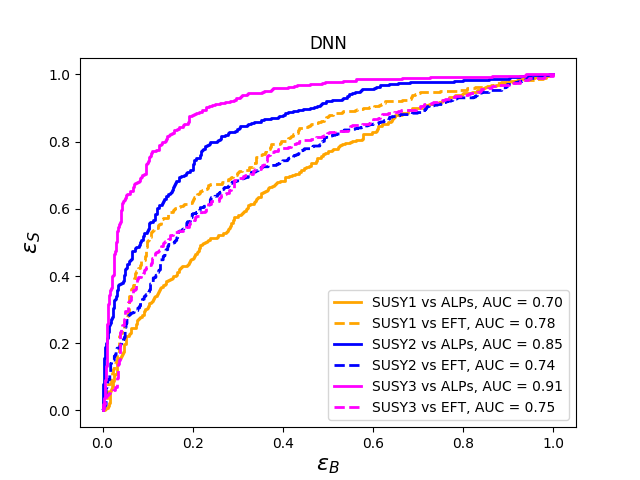
\includegraphics[scale=0.50]{draftfig/2D_DNN_SUSY_vs_sig_NLO_pt-metphij1_ROC.png}
\caption{ROC curves (DNN with 2D histograms, $r = 20$) for signal versus signal for the dijet NLO detector level simulation. For these plots, 40K events are used for each process in both the cases.}\label{2D_DNN_sig_vs_sig_NLO_ROC}
\end{figure}






\subsection{CNN}
We also used convolution neural network for the 2D histograms, with 2 convolution layers, 2 max-pooling layers and one dense 
flatten hidden layers, ReLu activation function for all the cases. The ROC curves for all the signals versus SM background are shown in fFgure \ref{2D_CNN_sig_vs_bg_LO_ROC} and the ROC curves for signal to signal are shown in Figure \ref{2D_CNN_SUSY_vs_sig_LO_ROC}. As mentioned earlier, although CNNs use the information of spatial correlations so usually perform better than DNNs for the image data. But in our case, because images are constructed from highly processed
information they do not enhance the performance. 


\begin{figure}% [H]
\centering
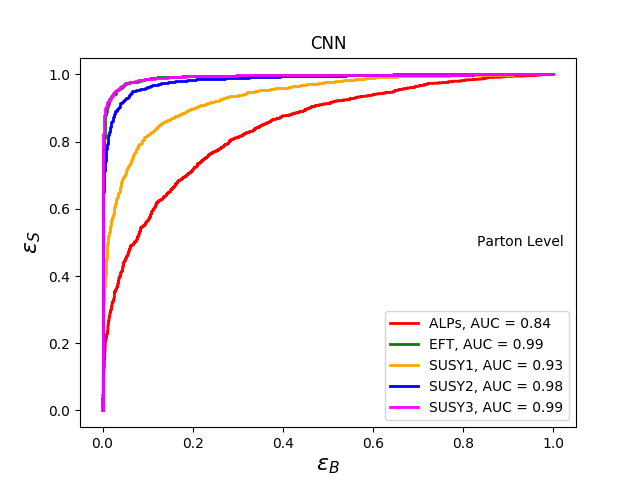
\includegraphics[scale=0.50]{draftfig/2D_CNN_sig_vs_bg_LO_ROC.png}
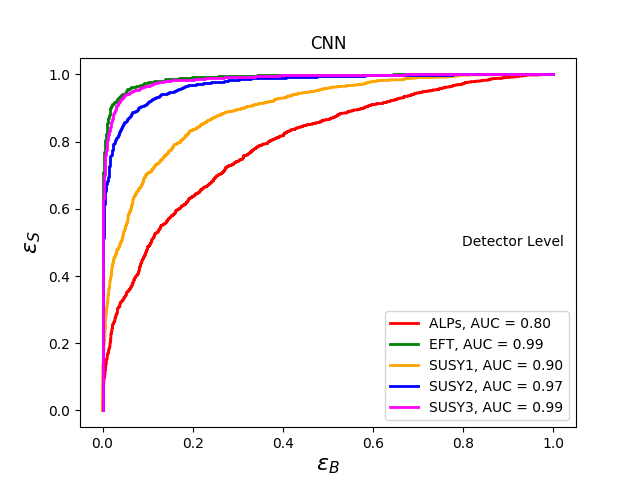
\includegraphics[scale=0.50]{draftfig/2D_CNN_sig_vs_bg_delphes_ROC.png}
\caption{ROC curves (CNN with 2D histograms, $r = 20$) for signal versus background for the parton level(left panel) and detector level simulation (right panel). For these plots, 100K events are used for each process in both the cases. For these plots, 100K events are used for each process in both the cases.}\label{2D_CNN_sig_vs_bg_LO_ROC}
\end{figure}

\begin{figure}% [H]
\centering
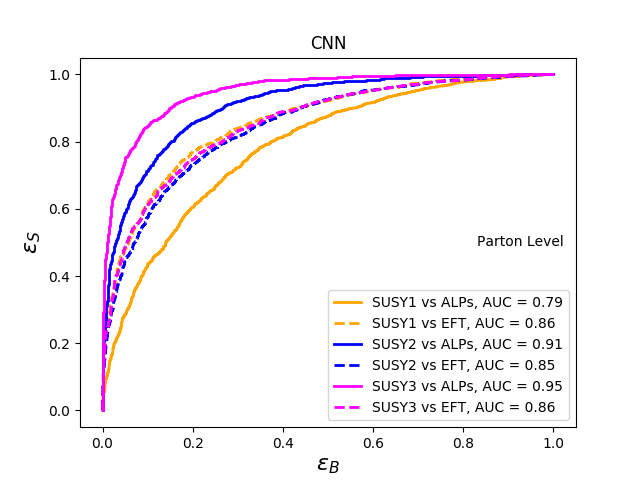
\includegraphics[scale=0.50]{draftfig/2D_CNN_SUSY_vs_sig_LO_ROC.png}
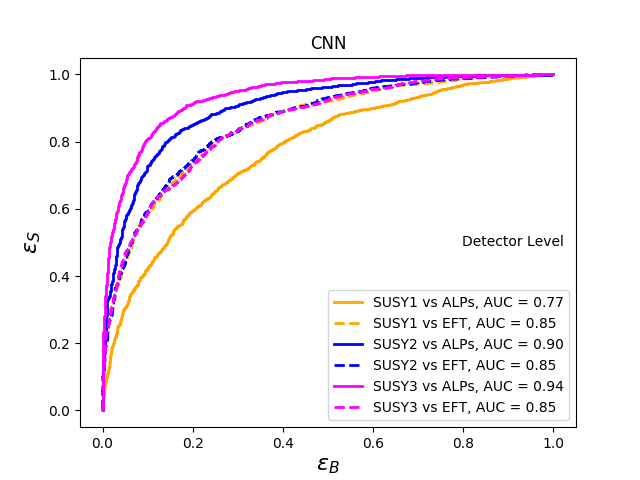
\includegraphics[scale=0.50]{draftfig/2D_CNN_SUSY_vs_sig_delphes_ROC.png}
\caption{ROC curves (CNN with 2D histograms, $r = 25$) for SUSY benchmarks versus other signals for the parton level(left panel) and detector level simulation (right panel).}\label{2D_CNN_SUSY_vs_sig_LO_ROC}
\end{figure}

The ROC curves for signal to background identification are shown in Figure \ref{2D_CNN_sig_vs_bg_NLO_ROC} and the ROC curves for signal to signal identification are shown in Figure \ref{2D_CNN_sig_vs_sig_NLO_ROC}.

\begin{figure}% [H]
\centering
\includegraphics[scale=0.50]{draftfig/2D_CNN_sig_vs_bg_NLO_pt-metphij1_ROC.png}
\caption{ROC curves (DNN with 2D histograms, $r = 20$) for signal versus background for the dijet NLO detector level simulation. For these plots, 40K events are used for each process in both the cases.}\label{2D_CNN_sig_vs_bg_NLO_ROC}
\end{figure}

\begin{figure}% [H]
\centering
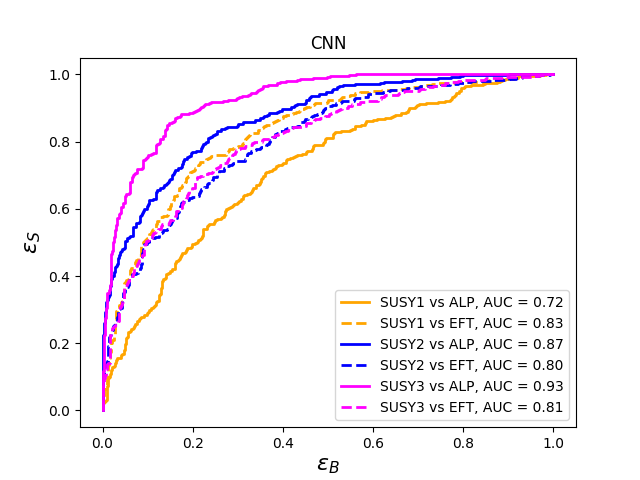
\includegraphics[scale=0.50]{draftfig/2D_CNN_SUSY_vs_sig_NLO_pt-metphij1_ROC.png}
\caption{ROC curves (DNN with 2D histograms, $r = 20$) for signal versus signal for the dijet NLO detector level simulation. For these plots, 40K events are used for each process in both the cases.}\label{2D_CNN_sig_vs_sig_NLO_ROC}
\end{figure}



We used the ML algorithms described in the previous section for monojet data. In figure \ref{rocLO-LR-NN}, ROC 
curves for different monojet signals are shown using LR and NN.
We can see that NN performs better than logistic regression. A balanced data set is considered for all the 
classes. We do not take into account the cross-sections for different processes.
It is more difficult to identify axion monojet final state from the SM background. Heavy WIMP is easy to distinguish. In this section, we also compared the 
classification accuracy for the parton level and fast detector simulation. In the actual detector environment, there is degradation in the performance.

\section{DM Characterization}
In the previous section, we discuss the identification of different monojet signals. It is found that heavy WIMPs and EFT monojet signals are easy
to distinguish from the SM background. The next question arises, is it possible to misidentify axion or EFT signal as WIMP. We use NN with kinematic features as input for the 
classification of different signals. As we have seen in the previous section, classification accuracy is not very different for the detector level simulated data. We consider parton level data for the purpose. The architecture of NN is same as previous section analysis. In figure
\ref{result2} we show the ROC curves for the  WIMP signal assuming other new physics signals as background. We consider 3 benchmark values for
the neutralino mass in the WIMP scenario. ROC AUC for WIMP BP3 versus eft and WIMP BP1 versus axion signal are 0.50 and 0.58 respectively. Therefore the
likelihood to confusing light WIMPs and axions is very high and the same is true for heavy WIMP and EFT monojet signal. This is shown in figure \ref{result3}. The likelihood is considered as false positive rate for the optimal point on the ROC curve. Since we are not considering the weightage of the cross-section for diffrent signals, we find optimal point by minimizing the Euclidean distance from the (1=tpr,0=fpr) value.


For DM identification also we use 2D histograms of $p_T$ and $\eta$ of the jet. As discussed in the previous section for signal versus background, in this case also averaging over more number of events per image  improves the classification accuracy. As an example, in figure \ref{accuracy1}, we show the accuracy plot for SUSY BP1 versus ALPs data. We are providing the information of approximate or exact likelihood function to NN depending on how many events per image are considered. We also check the accuracy dependence on the size of data sample. Once we have enough data to train the NN, having more events do not help. 
ROC curves for signal to signal identification using DNN are shown in figure \ref{2D_DNN_SUSY_vs_sig_LO_ROC}for the parton level and detector level simulation. {\textbf{WHY performance for detector level simulation is better than PL?}}. The ROC curves using CNN are shown in figure \ref{2D_CNN_SUSY_vs_sig_LO_ROC}. 

\begin{figure}% [H]
\centering
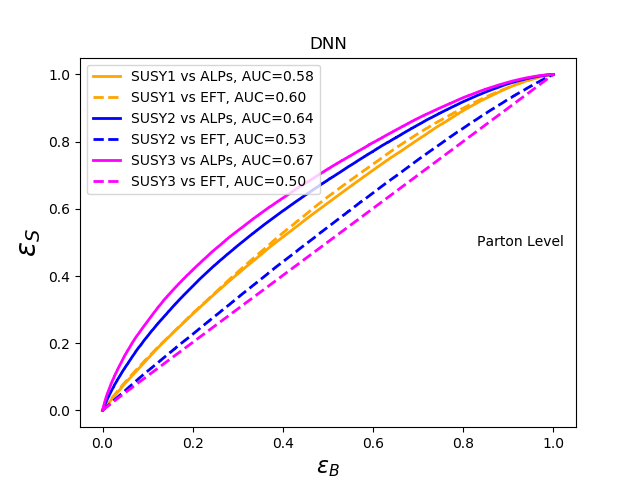
\includegraphics[scale=0.55]{draftfig/ROCssNN.png}
\caption{ROC curves using neural network (with 5 hidden layers) for different WIMP versus axion/EFT signal (LO parton level analysis). 
}\label{result2}
\end{figure}



\begin{figure}% [H]
\centering
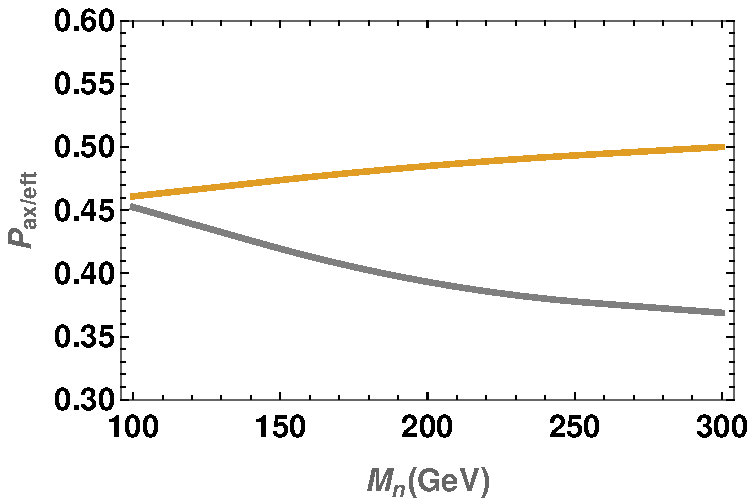
\includegraphics[scale=0.80]{draftfig/fprsusy-axioneft.pdf}
\caption{Probability of misidentifying axion(grey) or eft scenario (yellow curve) as WIMP, as a function of neutralino mass.}\label{result3}
\end{figure}




 
\begin{figure}% [H]
\centering
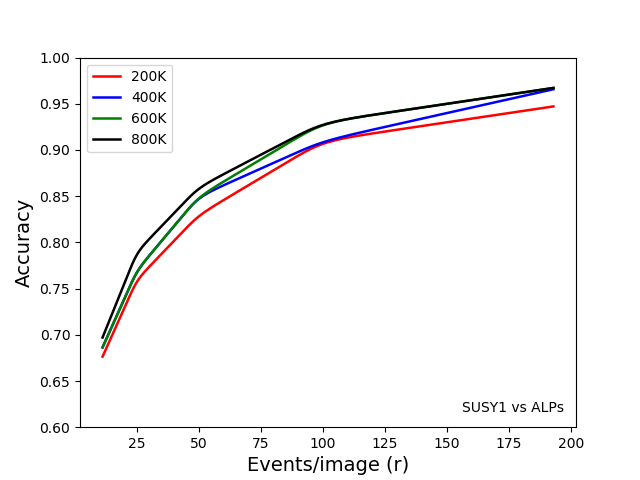
\includegraphics[scale=0.45]{draftfig/accuracyplot2dSUSY1vsAxion.pdf}
\caption{Accuracy versus no events per images with the varying number of events for WIMP BP1 versus ALPs using fully connected NN with 2 hidden layers. Red, blue,
green and black curves corresponding to a data sample of 200K, 400K, 600K, and 800K events.} \label{accuracy2}
\end{figure}



\begin{figure}% [H]
\centering
\includegraphics[scale=0.60]{draftfig/ROC2dAxionvsSUSY1.png}
\caption{ROC curve for $r=25$, $N=600K$ (fully connected NN with 2 hidden layers) events and 2d histograms (in a 29 $\times$ 29 grid) for SUSY-BP1 ans ALPS.}\label{roc2d}
\end{figure}

\section{NLO dijet}
For the NLO effect, we generate detector level events for the MET, monojet and dijet processes. For all the cases, we consider data sample of 40K events with one 
additional jet of $p_T>$ 25 GeV. 1D histograms for the constructed kinematic variable are shown in figure \ref{1Dand2DfeaturesDLdijet}. Additional jet provides us lot more 
information as compare to monojet. We use NN to analyze this data with 8 variables. Same as previous case, balanced data sample is considered for both the classes and data 
is divided into 70:30 proportion for the train and test sample. Architecture of NN is same as monojet case. We compare the classification accuracy for signal-background and 
signal-signal processes. The ROC curves for the same are shown in figure \ref{}. 



\begin{figure} [H]
\centering
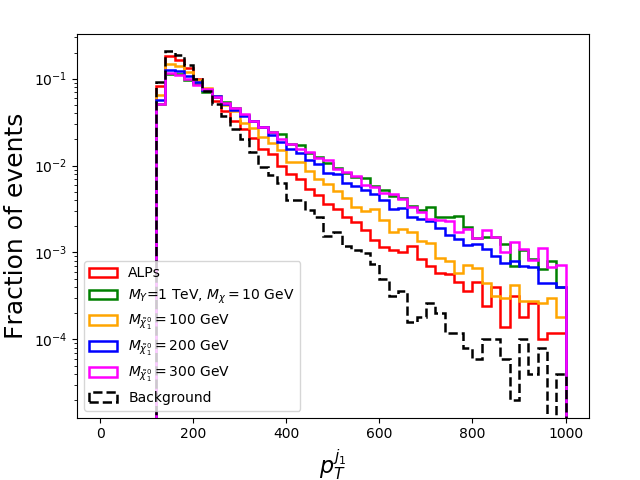
\includegraphics[scale=0.33]{draftfig/ptj1allsbdelphesdijet.png}
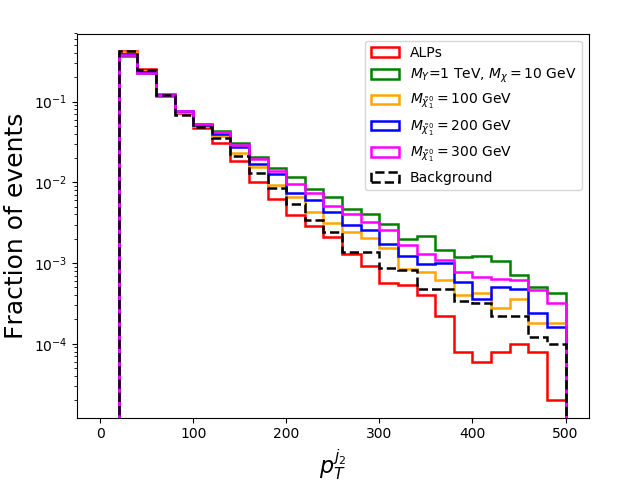
\includegraphics[scale=0.33]{draftfig/ptj2allsbdelphesdijet.png}
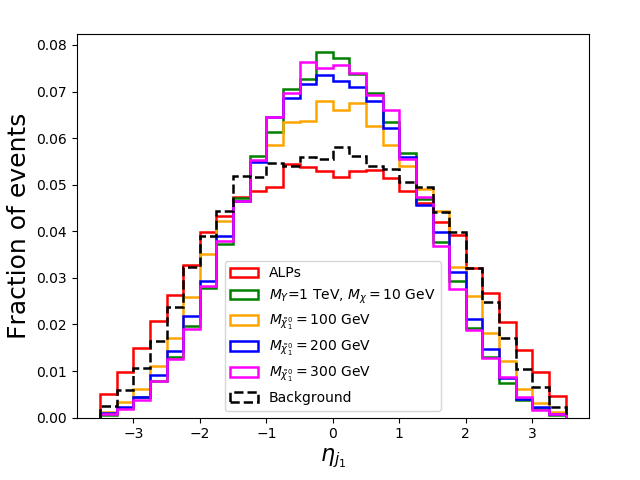
\includegraphics[scale=0.33]{draftfig/etaj1allsbdelphesdijet.png}
\includegraphics[scale=0.33]{draftfig/etaj2allsbdelphesdijet.png}
\includegraphics[scale=0.33]{draftfig/deltaphij1j2allsbdelphesdijet.png}
\includegraphics[scale=0.33]{draftfig/METallsbdelphesdijet.png}
\includegraphics[scale=0.33]{draftfig/deltaphiMETj1allsbdelphesdijet.png}
\includegraphics[scale=0.33]{draftfig/deltaphiMETj2allsbdelphesdijet.png}
\caption{1D histograms for the dijet process for linear ALPs, spin-1 mediator case, WIMP and SM background (detector simulation).\label{1Dand2DfeaturesDLdijet}}
\end{figure}


We apply  principle component analysis to dijet data sample. In figures \ref{}, \ref{}, \ref{} and \ref{}, we show the output for signal and background process.


\section{Conclusions and Outlook}
In this paper, we used supervised machine learning algorithms for the identification of WIMP dark matter in the monojet channel. For the kinematic variables, 
NN performs better than logistic regression. By constructing 2D histograms of $p_T$ and $\eta$ of the jet by averaging over several number of events. For the 
image data, we used both neural network and convolutional neural network. This method offers a better distinguish between between WIMP signal and other signals. 

We also investigate NLO process and find that accuracy increases in this case ...PCA analysis

For the monojet data, one could consider the jet images constructed event by event. Incorporating the information of cross-section ..
This analysis could be extended for other channels for collider dark matter searches. 
Unsupervised techniques...

\section{acknowledgments}
%\begin{acknowledgments}
C.K.K. wishes to acknowledge support from the Royal Society-SERB Newton International Fellowship (NF171488). 
The work of V.S. by the Science Technology and Facilities Council (STFC) under grant number
ST/P000819/1.
%\end{acknowledgments}

\appendix
%%%%%%%%%%%%%%%%%%%%%%%%%%%%%%%%%%%%%%%%%%%%%%%%%%%
\section{Analysis set-up\label{setup}}
%%%%%%%%%%%%%%%%%%%%%%%%%%%%%%%%%%%%%%%%%%%%%%%%%%%
We generate parton level events for mono jet and missing energy signal for centre of mass energy $\sqrt{s}=14$ TeV using MC$@$NLO
Madgraph. For SUSY WIMP, we used MSSM-SLHA2 model, for linear axion like particle(ALP) feynrule model available 
in the literature\cite{linearalps} and DMSimp\cite{} model for spin 1 mediator in EFT set-up. For all the processes 400K events are generated.
A cut of $p_T^j > 130$ GeV and following kinematical variables are constructed
\[ Monojet : p_T^j (MET) ,\eta_j, \phi_j  \]
SM dominant monojet background:
\be  pp \rightarrow Z j (Z \rightarrow \nu\bar\nu) \ee
For the detector simulation, atlas card and Delphes.. is used. For this case 100K events are generated for both the processes. 
For the  NLO monojet signal. A cut of $p_T^j > 130$ GeV for leading jet $p_T$ and $p_T^j > 25$ GeV  for sub-leading jet is implemented both at the generation 
level and while analysing the root file. To avoid the double counting from parton shower and matrix element method, jet merging scheme (MLM)
with xqcut 20 GeV. For the monojet we again have three kinematic features same as parton level monojet events. For the dijet, we 
construct following kinematic variables :
\[ p_T^{j_1}, p_T^{j_2}, \eta_{j_1}, \eta_{j_2}, MET, \Delta \phi_{jj}, \Delta \phi_{MET j_1}, \Delta \phi_{MET j_2} \]
here $j_1$ and $j_2$ refer to the leading and sub-leading jet respectively. For the di-jet sample we analyze data sample of 40 K events for all the processes.


\section{PCA correlations\label{PCA}}

\begin{table}
\centering
\scalebox{0.55}{
\begin{tabular}{|c|c|c|c|c|c|c|c|c|}
\hline
\multicolumn{9}{|c|}{Background PCA correlations} \\
\hline
\toprule
{} &  $p_T^{j_1}$ &  $p_T^{j_2}$ &  $\eta_{j_1}$ &  $\eta_{j_2}$ &  $\Delta \phi_{jj}$ &   $\text{MET}$ &  $\Delta \phi_{\text{MET}}^{j_1}$ &  $\Delta \phi_{\text{MET}}^{j_2}$ \\ \hline
\midrule
PC-1 &  0.09 &  0.03 &  -0.01 &  -0.01 &  -0.63 &  0.08 &      0.74 &      0.20 \\ \hline
PC-2 &  0.74 &  0.25 &  -0.00 &   0.01 &   0.08 &  0.61 &     -0.09 &     -0.02 \\ \hline
PC-3 & -0.01 & -0.06 &   0.63 &   0.63 &   0.21 &  0.03 &      0.09 &      0.38 \\ \hline
PC-4 &  0.01 &  0.05 &   0.31 &   0.31 &  -0.44 & -0.03 &     -0.17 &     -0.76 \\ \hline
PC-5 &  0.14 &  0.84 &   0.02 &   0.03 &   0.04 & -0.52 &      0.02 &      0.07 \\ \hline
PC-6 &  0.00 &  0.01 &   0.71 &  -0.71 &  -0.00 &  0.00 &      0.00 &     -0.00 \\ \hline
PC-7 & -0.65 &  0.48 &  -0.00 &   0.00 &   0.00 &  0.59 &     -0.00 &     -0.00 \\ \hline
PC-8 &  0.00 &  0.00 &  -0.00 &  -0.00 &   0.60 & -0.00 &      0.64 &     -0.48 \\ \hline
\bottomrule
\end{tabular}}
\scalebox{0.55}{
\begin{tabular}{|c|c|c|c|c|c|c|c|c|}
\hline
\multicolumn{9}{|c|}{ALP PCA correlations} \\
\hline
\toprule
{} &  $p_T^{j_1}$ &  $p_T^{j_2}$ &  $\eta_{j_1}$ &  $\eta_{j_2}$ &  $\Delta \phi_{jj}$ &   $\text{MET}$ &  $\Delta \phi_{\text{MET}}^{j_1}$ &  $\Delta \phi_{\text{MET}}^{j_2}$ \\ \hline
\midrule
PC-1 &  0.68 &  0.29 &  -0.00 &  -0.02 &  -0.01 &  0.67 &      0.00 &     -0.00 \\ \hline
PC-2 &  0.00 & -0.02 &   0.00 &   0.00 &  -0.45 &  0.00 &      0.77 &      0.46 \\ \hline
PC-3 &  0.01 & -0.01 &   0.03 &   0.03 &   0.71 &  0.01 &     -0.00 &      0.70 \\ \hline
PC-4 & -0.02 &  0.01 &  -0.71 &  -0.71 &   0.03 & -0.01 &      0.00 &      0.03 \\ \hline
PC-5 & -0.19 &  0.96 &   0.03 &  -0.01 &   0.00 & -0.22 &      0.01 &      0.02 \\ \hline
PC-6 & -0.00 & -0.03 &   0.71 &  -0.71 &  -0.00 & -0.00 &     -0.00 &     -0.00 \\ \hline
PC-7 &  0.71 & -0.03 &  -0.00 &  -0.00 &  -0.00 & -0.70 &     -0.00 &     -0.00 \\ \hline
PC-8 &  0.00 &  0.00 &   0.00 &  -0.00 &  -0.54 & -0.00 &     -0.64 &      0.54 \\ \hline
\bottomrule
\end{tabular}}
\scalebox{0.55}{
\begin{tabular}{|c|c|c|c|c|c|c|c|c|}
\hline
\multicolumn{9}{|c|}{EFT PCA correlations} \\
\hline
\toprule
{} &  $p_T^{j_1}$ &  $p_T^{j_2}$ &  $\eta_{j_1}$ &  $\eta_{j_2}$ &  $\Delta \phi_{jj}$ &   $\text{MET}$ &  $\Delta \phi_{\text{MET}}^{j_1}$ &  $\Delta \phi_{\text{MET}}^{j_2}$ \\ \hline
\midrule
PC-1 &  0.68 &  0.31 &   0.00 &  -0.00 &   0.02 &  0.66 &     -0.02 &     -0.01 \\ \hline
PC-2 &  0.01 &  0.02 &   0.01 &  -0.03 &  -0.37 &  0.01 &      0.76 &      0.53 \\ \hline
PC-3 &  0.01 &  0.02 &  -0.04 &  -0.01 &  -0.77 & -0.00 &      0.07 &     -0.63 \\ \hline
PC-4 &  0.00 & -0.00 &  -0.71 &  -0.71 &   0.03 &  0.00 &     -0.01 &      0.02 \\ \hline
PC-5 & -0.16 &  0.95 &  -0.01 &   0.00 &   0.02 & -0.28 &     -0.02 &      0.00 \\ \hline
PC-6 & -0.00 &  0.00 &   0.71 &  -0.71 &  -0.01 & -0.00 &     -0.02 &     -0.03 \\ \hline
PC-7 &  0.72 & -0.08 &   0.00 &  -0.00 &   0.00 & -0.69 &      0.00 &      0.00 \\ \hline
PC-8 &  0.00 & -0.00 &  -0.00 &  -0.00 &   0.52 & -0.00 &      0.64 &     -0.56 \\ \hline
\bottomrule
\end{tabular}}
\vspace{0.7cm}

\scalebox{0.55}{
\begin{tabular}{|c|c|c|c|c|c|c|c|c|}
\hline
\multicolumn{9}{|c|}{SUSY $M_{\tilde{\chi}} = 100$ GeV PCA correlations} \\
\hline
\toprule
{} &  $p_T^{j_1}$ &  $p_T^{j_2}$ &  $\eta_{j_1}$ &  $\eta_{j_2}$ &  $\Delta \phi_{jj}$ &   $\text{MET}$ &  $\Delta \phi_{\text{MET}}^{j_1}$ &  $\Delta \phi_{\text{MET}}^{j_2}$ \\ \hline
\midrule
PC-1 &  0.69 &  0.28 &  -0.01 &  -0.01 &  -0.00 &  0.67 &      0.02 &      0.02 \\ \hline
PC-2 &  0.02 & -0.00 &  -0.01 &   0.00 &   0.24 &  0.02 &     -0.74 &     -0.62 \\ \hline
PC-3 & -0.01 & -0.01 &  -0.71 &  -0.71 &   0.01 & -0.01 &      0.00 &      0.01 \\ \hline
PC-4 & -0.00 &  0.02 &  -0.01 &  -0.01 &  -0.85 & -0.00 &      0.15 &     -0.50 \\ \hline
PC-5 & -0.14 &  0.96 &   0.00 &  -0.01 &   0.02 & -0.26 &     -0.01 &      0.00 \\ \hline
PC-6 & -0.01 &  0.01 &  -0.71 &   0.71 &  -0.00 & -0.00 &      0.01 &      0.00 \\ \hline
PC-7 & -0.71 &  0.09 &   0.00 &  -0.00 &   0.00 &  0.69 &     -0.00 &     -0.00 \\ \hline
PC-8 &  0.00 & -0.00 &   0.00 &   0.00 &   0.47 &  0.00 &      0.65 &     -0.60 \\ \hline
\bottomrule
\end{tabular}}
\scalebox{0.55}{
\begin{tabular}{|c|c|c|c|c|c|c|c|c|}
\hline
\multicolumn{9}{|c|}{SUSY $M_{\tilde{\chi}} = 200$ GeV PCA correlations} \\
\hline
\toprule
{} &  $p_T^{j_1}$ &  $p_T^{j_2}$ &  $\eta_{j_1}$ &  $\eta_{j_2}$ &  $\Delta \phi_{jj}$ &   $\text{MET}$ &  $\Delta \phi_{\text{MET}}^{j_1}$ &  $\Delta \phi_{\text{MET}}^{j_2}$ \\ \hline
\midrule
PC-1 &  0.68 &  0.29 &   0.00 &   0.00 &   0.02 &  0.67 &     -0.07 &     -0.06 \\ \hline
PC-2 &  0.07 &  0.02 &   0.01 &   0.01 &  -0.23 &  0.07 &      0.74 &      0.62 \\ \hline
PC-3 &  0.01 & -0.02 &  -0.13 &  -0.13 &  -0.84 &  0.01 &      0.16 &     -0.49 \\ \hline
PC-4 &  0.01 & -0.02 &  -0.70 &  -0.70 &   0.15 &  0.01 &     -0.02 &      0.10 \\ \hline
PC-5 & -0.17 &  0.96 &   0.00 &  -0.04 &  -0.02 & -0.24 &      0.01 &     -0.00 \\ \hline
PC-6 & -0.00 &  0.03 &  -0.71 &   0.71 &  -0.00 & -0.01 &      0.00 &      0.00 \\ \hline
PC-7 & -0.71 &  0.05 &  -0.00 &   0.00 &  -0.00 &  0.70 &     -0.00 &     -0.00 \\ \hline
PC-8 &  0.00 &  0.00 &   0.00 &   0.00 &   0.47 & -0.00 &      0.65 &     -0.60 \\ \hline
\bottomrule
\end{tabular}}
\scalebox{0.55}{
\begin{tabular}{|c|c|c|c|c|c|c|c|c|}
\hline
\multicolumn{9}{|c|}{SUSY $M_{\tilde{\chi}} = 300$ GeV PCA correlations} \\
\hline
\toprule
{} &  $p_T^{j_1}$ &  $p_T^{j_2}$ &  $\eta_{j_1}$ &  $\eta_{j_2}$ &  $\Delta \phi_{jj}$ &   $\text{MET}$ &  $\Delta \phi_{\text{MET}}^{j_1}$ &  $\Delta \phi_{\text{MET}}^{j_2}$ \\ \hline
\midrule
PC-1 &  0.70 &  0.16 &  -0.00 &   0.01 &   0.00 &  0.69 &     -0.01 &     -0.01 \\ \hline
PC-2 &  0.01 &  0.01 &   0.00 &   0.00 &  -0.31 &  0.01 &      0.75 &      0.58 \\ \hline
PC-3 & -0.00 &  0.01 &   0.71 &   0.71 &  -0.05 & -0.00 &      0.00 &     -0.04 \\ \hline
PC-4 &  0.00 &  0.01 &   0.04 &   0.04 &   0.81 &  0.00 &     -0.10 &      0.57 \\ \hline
PC-5 & -0.08 &  0.99 &  -0.01 &  -0.01 &  -0.00 & -0.15 &     -0.01 &     -0.01 \\ \hline
PC-6 &  0.00 &  0.00 &   0.71 &  -0.71 &  -0.00 &  0.00 &     -0.00 &     -0.00 \\ \hline
PC-7 &  0.71 & -0.05 &  -0.00 &   0.00 &   0.00 & -0.70 &      0.00 &      0.00 \\ \hline
PC-8 &  0.00 &  0.00 &  -0.00 &   0.00 &   0.49 & -0.00 &      0.65 &     -0.58 \\ \hline
\bottomrule
\end{tabular}}

\caption{PCA original feature to principal component correlations (rounded to 2 d.p.)}
\end{table}\label{PCA_table}



\begin{thebibliography}{99}
\bibitem{linearalps} 
http://feynrules.irmp.ucl.ac.be/wiki/ALPsEFT

\bibitem{Mimasu:2014nea}
  K.~Mimasu and V.~Sanz,
  %``ALPs at Colliders,''
  JHEP {\bf 1506} (2015) 173,
%  doi:10.1007/JHEP06(2015)173
  [arXiv:1409.4792 [hep-ph]].
  %%CITATION = doi:10.1007/JHEP06(2015)173;%%



\bibitem{Brivio:2017ije}
  I.~Brivio, M.~B.~Gavela, L.~Merlo, K.~Mimasu, J.~M.~No, R.~del Rey and V.~Sanz,
  %``ALPs Effective Field Theory and Collider Signatures,''
  Eur.\ Phys.\ J.\ C {\bf 77} (2017) no.8,  572,
%  doi:10.1140/epjc/s10052-017-5111-3
  [arXiv:1701.05379 [hep-ph]].
  %%CITATION = doi:10.1140/epjc/s10052-017-5111-3;%%
  %37 citations counted in INSPIRE as of 08 Mar 2019


%\cite{Freitas:2019hbk}
\bibitem{Freitas:2019hbk}
  F.~F.~Freitas, C.~K.~Khosa and V.~Sanz,
  %``Exploring SMEFT in VH with Machine Learning,''
  arXiv:1902.05803 [hep-ph].
  %%CITATION = ARXIV:1902.05803;%%

\end{thebibliography}

\end{document}


%\begin{figure} [H]
%\centering
%\caption{ROC curves (DNN with 2D histograms, $r = 25$) for signal versus background for the detector level simulation}\label{2D_DNN_sig_vs_bg_delphes_ROC}
%\end{figure}
%\begin{figure} [H]
%\centering
%\caption{ROC curves (CNN with 2D histograms, $r = 25$) for signal versus background for the detector level simulation}\label{2D_CNN_sig_vs_bg_delphes_ROC}
%\end{figure}
%\begin{figure} [H]
%\centering
%\caption{ROC curves (DNN with 2D histograms, $r = 25$) for SUSY benchmarks versus other signals for the detector level simulation}\label{2D_DNN_SUSY_vs_sig_delphes_ROC}
%\end{figure}
%\begin{figure} [H]
%\centering
%\caption{ROC curves (CNN with 2D histograms, $r = 25$) for SUSY benchmarks versus other signals for the detector level simulation}\label{2D_CNN_SUSY_vs_sig_delphes_ROC}
%\end{figure}




\begin{figure} [H]
\centering
\includegraphics[scale=0.30]{draftfig/axion/dijet/ptj1axspin1.png}
\includegraphics[scale=0.30]{draftfig/axion/dijet/ptj2axspin1.png}
\includegraphics[scale=0.30]{draftfig/axion/dijet/etaj1axspin1.png}
\includegraphics[scale=0.30]{draftfig/axion/dijet/etaj2axspin1.png}
\includegraphics[scale=0.30]{draftfig/axion/dijet/metaxspin1.png}
\includegraphics[scale=0.30]{draftfig/axion/dijet/deltaphijjaxspin1.png}
\includegraphics[scale=0.30]{draftfig/axion/dijet/dphimetj1axspin1.png}
\includegraphics[scale=0.30]{draftfig/axion/dijet/dphimetj2axspin1.png}
\caption{Linear ALPs, di-jet(parton level)}
\end{figure}



%\begin{figure} [H]
%\centering
%\includegraphics[scale=0.60]{draftfig/acVsNevents.pdf}
%\caption{Accuracy versus number of images with varying number of events (fully connected NN with 2 hidden layers) in a 29 $\times$ 29 grid.}\label{accuracy2}
%\end{figure}



%\begin{figure} [H]
%\centering
%\includegraphics[scale=0.40]{draftfig/ROCsignalLRandNN.png}
%\caption{ROC curves using logistic regression and neural network (with 10 hidden layers) for ALPs versus EFT and ALPs versus WIMPs (LO parton level analysis).}
%\end{figure}


%\section{Unsupervised learning}

\section{Need to understand}
What is the correct approach to use multi-dimensional probability information ?

What about the density estimates which experimentalists were discussing at ICTP workshop.


for this project we will also provide number of parameters information.


	\item . We could find $\sigma_\mathrm{LO}^\mathrm{1j}/\sigma_\mathrm{NLO}^\mathrm{2j}$ (why is this useful?) and also use backgrounds (mostly p p $>$ Z j with p p $>$ W j) - given in \cite{Barducci:2015ffa}. 
	


